\subsection{Visual Research Focus}


\paragraph{Speakers/Coordinators:} Marion M�ller and Peter Ludes

\vspace{0.6cm}
Two specific long-term IUB-research groups center on visuals and their communication: (1) founded and chaired by Prof. Peter Ludes since 2003, researchers from within IUB and from the outside have been studying collective visual memories and neglections as they emerged in various cultures, with trans-cultural and global elements; (2) initiated and co-ordinated by Prof. Marion G. M�ller in 2004, a transdisciplinary research group on "Visual Competence" scrutinizes the perception, dissemination, communication, interpretation and reception of visuals in contemporary societies. Both IUB-research groups work closely together and share partially overlapping interests, but are interested in different aspects of visual communication, using different methodological and theoretical approaches.

\vspace{0.6cm}
\textbf{(1) Visual Memories}\\
Visual memories are systematized and decoded by means of the concept of "key" visuals, which encompasses visual images and stereotypes. The focus is placed on key visuals in the media systems of the contemporary military, political and media superpower of the United States, set into contrast with Germany, Brazil, i.e., the potential leading power of Latin America (with one of the world's biggest TV stations and significant export quota) and the uprising world power of China. By means of a comparison between selected media, in their cultural contexts, over the period of about a decade, we inquire into the accelerating Americanization, visualization and globalization of screen media. The analysis and interpretation of the vast amount of visual data from television, web offerings and those transmitted via mobile devices requires cooperation with specialists in semi-automatic picture retrieval and information management. Our cooperation aims at the specification of culture-specific vs. trans-cultural visualization patterns. A systematic sample of TV programs and web offerings from Brazil, China, Germany and the United States as well as a model of common categories for analysis, statistical tools and devices for semi-automatic picture retrieval allows for a coherent research network. These projects from the SHSS (and Prof. Herzog from the Centre of Computing Technologies at the University of Bremen) cooperate with further projects at the universities of Kassel (Prof. Noeth) and Constance (Prof. Kramer) as well as at the universities of Bergen (Prof. Gripsrud, on the digitisation of audio-visual culture), and Salvador da Bahia (Prof. Boccia, on the complementarity of key measures and key visuals). In January 2006 we organized a workshop on Modelling and Decoding of Key Visuals in Intercultural Comparisons. Our website www.keyvisuals.org informs about our activities.
\begin{figure}[ht]
  \begin{center}
    
\includegraphics[width=\linewidth]{./TransdResearch/VRF-fig1.jpg}
%   \mycaption{ xxx )}\label{fig:profxxx}
   \end{center}
\end{figure}\\

Participants: Within IUB: Profs. A. Kappas, P. Ludes, M.G. M�ller, W. Werner, A. Wilhelm, (all SHSS), W. Bergholz (SES). Outside collaborators include Profs. L. Boccia, Scenic Arts and Cultural Studies, Federal University of Bahia, J. Gripsrud, Media Studies, Bergen, O. Herzog, Centre of Computing Technologies, Universit\"at Bremen, S. Kramer, Media Studies, Universit\"at Konstanz, J. Maguire, Sport Sociology, Loughborough University, W. N\"{o}th, Cultural Studies, Universit\"at Kassel.

\newpage
\textbf{(2) Visual Competence}\\
One of the major activities of the IUB research group "Visual Competence" in 2006 was the drafting of an international symposium proposal - Visual Competence: Facets of a Paradigm Shift -, submitted in November to the Volkswagen-Foundation. The symposium with 32 internationally accomplished speakers is planned to be hosted at IUB (then: Jacobs University Bremen) in July 2007, bringing together international experts from the United States, Canada, Australia, Brazil, Great Britain, the Netherlands, Sweden and Germany to discuss the potential of the concept "Visual Competence" from a transdisciplinary perspective, featuring experts from communication science, art history, cognitive and media psychology, sociology and political science.
It is the intention of the research group to build on the discussions and critique at the symposium and submit a new proposal to the Deutsche Forschungsgemeinschaft (DFG) in October 2007 on establishing a Research Training Group (Graduiertenkolleg) "Visual Competence", the external participants of the symposium being external advisors and members of the Graduiertenkolleg, should its establishment be granted.
\begin{figure}[ht]
  \begin{center}
    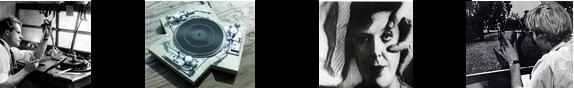
\includegraphics[width=\linewidth]{./TransdResearch/VRF-fig2.jpg}
%   \mycaption{ xxx )}\label{fig:profxxx}
   \end{center}
\end{figure}


The research group focuses on the study of four key aspects of visual competence: visual production competence, visual perception competence, visual reception competence, and multimodal/intercultural action competence. The research groups' logo - four images presented above - are symbolizing these four competences. The images are from left to right. (1) Analog film editing (production competence, anonymous source), (2) Sean Duffy, Thank You Ernest, JoJo \& Leslie, 2003 (multimodal action competence), (3) Filmstill from Luis Bu�uel, Un Chien Andalou, 1929 (perception competence), (4) Filmstill Michelangelo Antonioni, Blow Up, 1966 (reception competence).

\vspace{0.6cm}
A specific research project in the context of the Visual Research Focus "Visual Competence" is "Perceiving Press Photography: Who Sees What, When, How?" conducted by psychologists Prof. Bettina Olk and Prof. Arvid Kappas and mass communication Prof. Marion G. M�ller. In this transdisciplinary project, the perception, meaning attribution and reception of press photographs are tested in order to find out, how individuals, but also how different groups of participants (different gender, different social, national and cultural background) perceive and interpret contemporary news photographs depicting or relating to violent world events, and how they emotionally react to the same images.

\vspace{0.6cm}
IUB-members of Visual Competence research group (in alphabetical order): Profs. M. Bogaards, P. Crowther, J. F�rster, A. Kappas, U. K�hnen, P. Ludes, M. G. M�ller, B. Olk, H. Wessler, A. Wilhelm.

\vspace{0.6cm}
External invitees to the Visual Competence symposium and potential advisors and members of the Visual Competence research group (in order of appearance in the program): Profs. P. Messaris (University of Pennsylvania, Annenberg School, USA), J. Elkins (School of the Art Institute Chicago, USA), R. Hobbs (Temple University, USA), G. Kress (University of London, UK), M. Griffin (Carleton College, USA), K. Ritzenhoff (Central Connecticut State University, USA), T. Knieper (Ludwig Maximilians Universit�t M�nchen), H. Bredekamp (Humboldt-Universit�t zu Berlin), A. Kingstone (University of British Columbia in Vancouver, Canada), D. Glaser (The Wellcome Trust, UK), E. Tan (Universiteit van Amsterdam, Netherlands), F. Schwab/D. Unz (Universit�t Saarbr�cken), K. Holmqvist/J. Holsanova (University Lund, Sweden), T. van Leeuwen (University of Technology, Sydney, Australia), W. N�th (Universit�t Kassel), D. Freedberg (Columbia University, USA), L. Boccia (Federal University of Bahia, Salvador, Brazil), U. Frohne (Universit�t K�ln), B. Zelizer (University of Pennsylvania, Annenberg School, USA), M. Kraidy (American University, Washington D.C.), L. Santaella Braga (Catholic University of Sao Paulo, Brazil), M. Bruhn (Helmholtz-Zentrum, Berlin), C. M. Wolf (Universit�t Innsbruck, Austria), E. Grittmann (Universit�t Hamburg), B. Drechsel (Ludwig Boltzmann Institute for European History and Public Spheres, Gie�en), S. Baringhorst (Universit�t Siegen).
